\documentclass{article}

\usepackage{mhchem}
\usepackage{siunitx}
\usepackage{graphicx}
\usepackage{caption}
\usepackage{amsmath}
\usepackage{amsfonts}
\usepackage{physics}
\usepackage{url}

\newcommand{\cc}{$\,\text{cm}^{3}$}
\newcommand{\circa}{\emph{circa }}
\newcommand{\g}{\,g}

\title{Macroscopic AFM -- Results}
\date{01/12/2020}
\author{Samuel Frost}

\begin{document}

\maketitle

\section*{Results}
\subsection*{Fundamental frequency}
$b$, $d$ and $l$ were measured to be 3.65 $\pm 0.005$ mm, 1.59 $\pm 0.005$ mm and 232$\pm 1$ mm respectively. 
A micrometer was used to record the values for $b$ and $d$ so 
its error is relatively small, $\pm 0.005$\,mm, for $l$ however a ruler was used, giving a larger error of 
$\pm 1$\,mm, this is still low however.
The calculated value of $f_1$ was then determined to be 24.45 $\pm$ 2.32\,Hz.

The fundamental frequency resonance curve was plotted, using this calculated value as rought starting point.
The uncertainty in the frequency and amplitude were too low to see on the graph.
$$f_1 = 21.07\text{\,Hz}$$
The amplitude of $f_1$ is roughly 25\,cm, so for Q the bandwidth was calculated at 17.67\,cm.
$$Q = \frac{21.07}{21.33-20.85} = 43.896$$

\begin{tabular}{l | l}
    Frequency $\pm$ 0.005/ Hz & Amplitude $\pm 0.1$ / cm\\
    \hline
    12.19 & 0.4\\
    14.12 & 0.5\\
    17.01 & 1.1\\
    18.09&1.5\\
    18.43&1.6\\
    19.05&2\\
    19.31&2.2\\
    19.83&2.9\\
    20.05&3.3\\
    20.15&3.7\\
    20.35&4.5\\
    20.46&5.1\\
    20.67&7.6\\
    20.85&17.8\\
    21.07&24.9\\
    21.14&22.3\\
    21.31&17.5\\
    21.58&9.2\\
    21.80&6.2\\
    22.01&4.9\\
    22.68&2.7\\
    23.05&2.1\\
    23.66&1.7\\
\end{tabular}

\begin{figure}[h]
    \centering
    \captionsetup{justification=centering}
    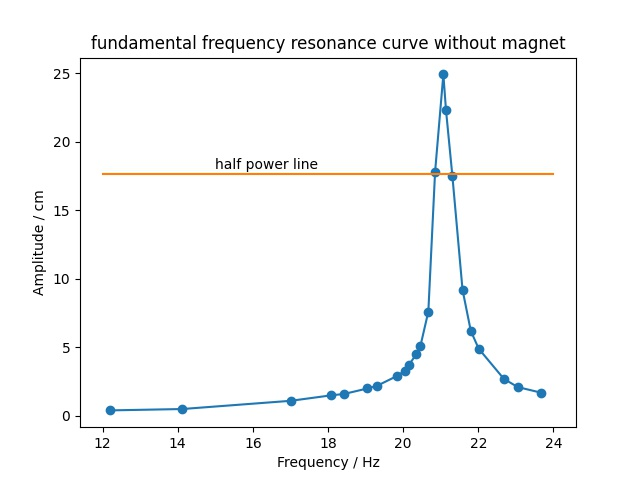
\includegraphics[width=12cm]{10.jpg}
    \caption{Resonance frequency curve of $f_1$ \label{f1}}
\end{figure}

The error of the frequency recorded is dependent upon the oscillator, it measures to 2 d.p. so the absolute
error is $\pm 0.005$\,Hz. When measuring the amplitude the error is from my ability to accurately read the laser
on the graph paper, it could be faint and shakey at times giving a less accurate reading. It was divided 
into 1\,mm squares, however I would say the error is 1\,mm. Given these errors I would say that my data is 
trustworthy in that a curve was formed with a clear peak.

$f_1$ was smaller than expected, with a percentage error of 16\%. This is because the moment of inertia that's used for the frequency calculation
does not take into account the tip, magnet and mirror at the end of the cantilever, these decrease the moment of 
inertia making the frequency lower than calculated. 
\newpage
\subsection*{Fundamental frequency with magnet}
For the next step the magnet was moved under the tip, it appeared to push the tip upwards, this is repulsive. 
In Figure: \label{f2} it can be seen that the fundamental frequency is shifted to the right when the magnet is 
beneath it. This is due to the force of the magnet increasing the effective spring constant, giving it a slightly
higher fundamental frequency. The cantilever is "stiffer" and so it takes more energy to make it resonate. 
The Q value calculated from this was 44.28, this is higher than without the magnet, indicating that 
it would drop off slower.

\begin{figure}[h]
    \centering
    \captionsetup{justification=centering}
    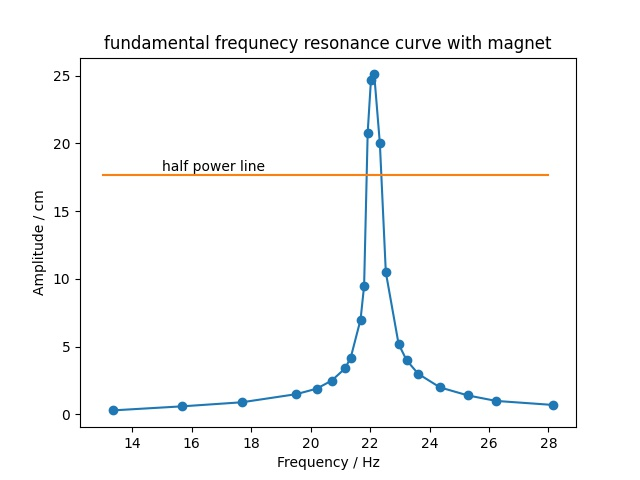
\includegraphics[width=12cm]{10_1.jpg}
    \caption{Resonance frequency curve of $f_1$ with a magnet\label{f2}}
\end{figure}

\newpage
\subsection*{Second harmonic frequency}
As seen in Figure: \label{f3} a clear fundamental frequency was obtained for the second harmonic frequency.
$f_2 =  141.9$\,Hz. The uncertainty in the frequency and amplitude is once again too low to see on the graph.
Q was found to be 126.517, this is much higher than for $f_1$, meaning that an oscillation inat $f_2$ would last 
for much longer. 
\begin{figure}[h]
    \centering
    \captionsetup{justification=centering}
    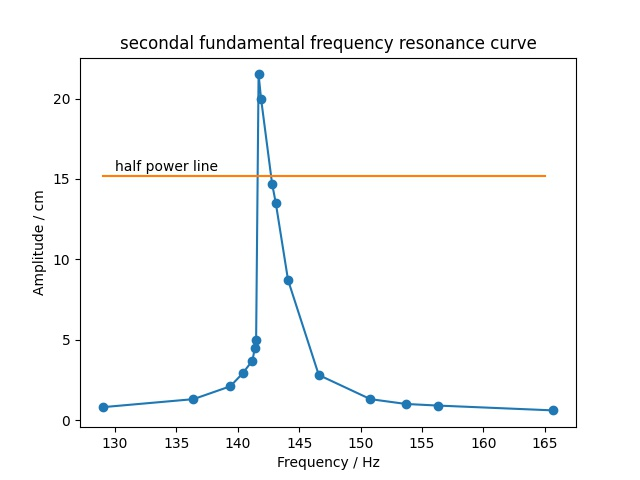
\includegraphics[width=12cm]{10_2.jpg}
    \caption{Resonance frequency curve of $f_2$\label{f3}}
\end{figure}

\end{document}


